\documentclass[11pt]{article}
\usepackage[margin=1in]{geometry}
\usepackage{booktabs}
\usepackage{amsmath}
\usepackage{graphicx}
\usepackage{hyperref}
\hypersetup{colorlinks=true, linkcolor=blue, urlcolor=blue}
\sloppy

\title{Recovering What Was Conditioned:\\
\large The content of the Planning Commission's conditions of approval}
\author{Dan Post}
\date{September 2026}

\begin{document}
\maketitle

\begin{abstract}
\noindent
The corpus memo's central pattern is a substitution: outright denial has fallen to
approximately zero while conditioning has more than tripled. The burden moved into the
\emph{content} of the approval. The dataset, as it stands, cannot see that content.
\texttt{conditions\_imposed} is populated on 25.9\% of items and its median length is three
characters --- it is the word ``yes''. The minutes record \emph{that} a project was
conditioned and almost never \emph{how}.

\medskip\noindent
This memo establishes where the content is and how much of it is obtainable. Four results.

\medskip\noindent
\textbf{The minutes do not hold it.} A regex sweep of all 25,927 source blocks finds 15 --- 
0.06\% --- that both name conditions and enumerate them, all from 1998--2001 and all
amendments announced from the dais. \textbf{DataSF does not hold it either}: there is no
commission-actions dataset, the two Planning Records tables carry applications rather than
decisions, and across DBI's 1,295,048 permit rows 87 mention a Commission condition or motion
at all.

\medskip\noindent
\textbf{The Commission packet does hold it}, and it is systematically addressable by case
number on two city hosts. On a stratified sample of 20 cases per hearing year, a packet exists
for 0\% of cases heard before 2010 and roughly 50--90\% of cases heard from 2011 on. The
packet carries the draft motion, whose \emph{Exhibit A --- Conditions of Approval} enumerates
and \emph{names} each condition. It is a conditional-use instrument: across every one of the 225
packets the probe found, \textbf{89 of 101 conditional-use cases} carry a conditions section
with a median of fifteen numbered, named conditions, against \textbf{1 of 41 discretionary
reviews}, because a DR produces a Discretionary Review Action rather than a conditioned
authorisation.

\medskip\noindent
\textbf{The conditions are templated, and a small scheme spans them.} The 225 packets yield
216 distinct condition headings over \textbf{1{,}622 impositions}, and a thirteen-category
keyword scheme --- split into conditions that change the \emph{project} and conditions that
change its \emph{obligations} --- reaches \textbf{85.6\% of those impositions} and 72.3\% of
the \texttt{modifications} field, the one place the existing dataset already holds condition
content. The split between the families is the sharpest result in the memo: weighted by how
often they are imposed, \textbf{58.4\% of staff's conditions change the project's obligations
and 12.8\% change the project}, while in the Commission's own amendments the proportions are
reversed.
\end{abstract}

\tableofcontents
\newpage

\section{The gap, stated precisely}

Three fields in the item table bear on conditions, and Table~\ref{tab:fields} is exact about
what each one is.

\begin{itemize}
\item \textbf{\texttt{conditions\_imposed}} is non-empty on \textbf{4{,}199 items (25.9\%)}. Of
those, 4{,}048 say \texttt{yes} and 151 say \texttt{no}. Its median length is three
characters. It is a flag.
\item \textbf{\texttt{project\_modified}} is \texttt{yes} on \textbf{1{,}403 items (8.7\%)}.
Also a flag, and orthogonal: 1{,}149 items are both conditioned and modified, 2{,}899
conditioned but not modified, 254 modified but not conditioned.
\item \textbf{\texttt{modifications}} carries free text on \textbf{1{,}735 items (10.7\%)},
median 108 characters. \emph{This is the one field in the dataset that holds condition
content}, and \S\ref{sec:modifications} treats it as such. 215 of those items do not have the
conditions flag set at all, which is a coding question worth a pass.
\end{itemize}

The extraction is not at fault here. It records what the minutes say, and the minutes say
``ACTION: Approved with conditions'' and then move on. Recovering content means going outside
the minutes.

\section{Where the conditions live: the instrument number}

The minutes do name the document that holds the conditions. Schema v2 records it:
\texttt{action\_instrument} $\in\{$\texttt{motion}, \texttt{resolution}, \texttt{dra}$\}$ and
\texttt{action\_instrument\_no}, the number.

% GENERATED BY analyze_conditions.py — do not edit by hand.
\begin{table}[htbp]\centering
\caption{The three fields in the item table that bear on conditions, over all 16{,}199 items. Only the third holds text.}\label{tab:fields}
\resizebox{\textwidth}{!}{%
\begin{tabular}{lrrl}\toprule
Field & Items & Share & What it holds\\\midrule
\texttt{conditions\_imposed} & 4,199 & 25.9\% & a flag: 4,048 \texttt{yes}, 151 \texttt{no}, median 3 characters\\
\texttt{project\_modified} & 1,403 & 8.7\% & a flag; 1,149 items are both conditioned and modified\\
\texttt{modifications} & 1,735 & 10.7\% & \textbf{free text}, median 108 characters\\
\quad \emph{\dots\ with no conditions flag set} & 215 & & a coding question worth a pass\\
\bottomrule\end{tabular}}\end{table}

\begin{table}[htbp]\centering
\caption{What the item table records about conditions, and how far the document number reaches. `Instrument' is \texttt{action\_instrument}; the number is \texttt{action\_instrument\_no}. Eras split at the 2015 change of document format.}\label{tab:instrument}
\resizebox{\textwidth}{!}{%
\begin{tabular}{lrrrr}\toprule
Items & $N$ & Conditions flag set & Instrument named & Number present\\\midrule
All & 16,199 & 25.0\% & 40.5\% & 39.5\%\\
1998--2014 (HTML) & 11,347 & 22.1\% & 37.1\% & 35.9\%\\
2015--2026 (PDF) & 4,852 & 31.7\% & 48.4\% & 47.7\%\\
\midrule
With conditions imposed & 4,048 & --- & 84.2\% & 82.9\%\\
\quad \emph{unreachable: conditions, no number} & 692 & & & 17.1\% \emph{of them}\\
\bottomrule\end{tabular}}\end{table}

\begin{table}[htbp]\centering
\caption{A regex sweep of all 25{,}927 source blocks --- the same text the extraction read. The minutes name the document that holds the conditions; they almost never hold the conditions.}\label{tab:sweep}
\resizebox{\textwidth}{!}{%
\begin{tabular}{lrr}\toprule
The block \dots & Blocks & Share\\\midrule
names a motion or resolution number & 5,997 & 23.13\%\\
says `conditions of approval' & 535 & 2.06\%\\
says `subject to the following conditions' & 0 & 0.00\%\\
refers to an Exhibit A & 24 & 0.09\%\\
carries an enumerated list of three or more items & 737 & 2.84\%\\
enumerates a condition (list + condition language) & 15 & 0.06\%\\
\bottomrule\end{tabular}}\end{table}

\begin{table}[htbp]\centering
\caption{Is a Commission packet published for the case? A stratified random sample of 20 cases per hearing year, HEAD-probed against both hosts. The packet carries the staff report and the draft motion, whose Exhibit A is the conditions of approval.}\label{tab:packets}
\begin{tabular}{lrrrr}\toprule
Hearing years & Probed & Packet found & Rate & Host\\\midrule
1998--2009 & 240 & 0 & 0\% & \texttt{---}\\
2010--2010 & 20 & 2 & 10\% & \texttt{s3}\\
2011--2016 & 120 & 91 & 76\% & \texttt{s3}\\
2017--2021 & 99 & 65 & 66\% & \texttt{s3}\\
2022--2026 & 99 & 67 & 68\% & \texttt{citypln, s3}\\
\midrule 2011--2026 & 318 & 223 & \textbf{70.1\%} & \\
All years & 578 & 225 & 39\% & \\
\bottomrule\end{tabular}\end{table}

\begin{table}[htbp]\centering
\caption{Of the packets pulled, which kinds of case carry a conditions section --- in a conditional-use motion, Exhibit A. A discretionary review normally does not: its packet is a staff analysis and its outcome is a Discretionary Review Action, not a conditioned authorisation, so the empty cell is the correct answer rather than a parser failure. `Not read' is packets the probe found but \texttt{fetch} has not opened; they are excluded from the rate rather than counted as negatives.}\label{tab:kinds}
\begin{tabular}{lrrrrr}\toprule
Case family & Pulled & Not read & Read & Conditions section & Median numbered\\\midrule
Conditional use & 101 & 0 & 101 & 89 & 15\\
Discretionary review & 41 & 0 & 41 & 1 & 5\\
Environmental & 7 & 0 & 7 & 0 & ---\\
Legislative & 25 & 0 & 25 & 1 & 0\\
Other & 42 & 0 & 42 & 13 & 17\\
Variance & 9 & 0 & 9 & 2 & 2\\
\midrule All & 225 & 0 & 225 & 106 & \\
\bottomrule\end{tabular}\end{table}

\begin{table}[htbp]\centering
\caption{The twenty most frequent condition headings across the 225 packets read, of which 103 yielded at least one numbered condition heading. The Commission's conditions are written from a template, and the template is the finding.}\label{tab:titles}
\resizebox{\textwidth}{!}{%
\begin{tabular}{lrlr}\toprule
Condition & Packets & Condition & Packets\\\midrule
Enforcement & 88 & Revocation due to Violation of Conditions & 84\\
Extension & 84 & Conformity with Current Law & 75\\
Validity & 74 & Community Liaison & 71\\
Expiration and Renewal & 70 & Sidewalk Maintenance & 62\\
Diligent Pursuit & 46 & Final Materials & 36\\
Bicycle Parking & 31 & Project Description & 28\\
Surrounding Properties and Neighborhood & 28 & Site Description and Present Use & 27\\
Planning Code Compliance & 26 & Garbage, composting and recycling storage & 24\\
Planning Code Section 101 & 24 & Diligent pursuit & 24\\
Garbage, Composting and Recycling Storage & 24 & General Plan Compliance & 23\\
\bottomrule\end{tabular}}\end{table}

\begin{table}[htbp]\centering
\caption{A thirteen-category scheme, tested against the two sources of condition text that exist: the numbered condition headings of the packet motions (216 distinct headings over 1622 occurrences) and the \texttt{modifications} field of the item table ($N=1735$ items). Headings are reported both by distinct heading and weighted by how often each is imposed; the weighted column is the share of \emph{conditions} the scheme reaches. Categories are indicators, not a partition: one condition can carry two.}\label{tab:taxonomy}
\resizebox{\textwidth}{!}{%
\begin{tabular}{llrrr}\toprule
Family & Category & \multicolumn{2}{c}{Packet condition headings} & Minutes modifications\\
\cmidrule(lr){3-4} & & distinct & weighted & \\\midrule
Changes the project & Massing and envelope & 0.9\% & 0.2\% & 28.5\%\\
 & Unit count and mix & 1.9\% & 0.4\% & 5.2\%\\
 & Design and materials & 6.9\% & 7.4\% & 25.9\%\\
 & Use and operations & 9.3\% & 4.9\% & 8.8\%\\
\midrule
Changes its obligations & Affordability & 3.2\% & 0.6\% & 3.6\%\\
 & Fees and exactions & 3.7\% & 2.9\% & 2.3\%\\
 & Transport and parking & 7.4\% & 8.9\% & 12.4\%\\
 & Open space and streetscape & 3.2\% & 5.3\% & 5.7\%\\
 & Monitoring and reporting & 8.3\% & 21.2\% & 11.7\%\\
 & Environmental mitigation & 0.9\% & 0.4\% & 2.9\%\\
 & Historic preservation & 0.9\% & 0.1\% & 2.1\%\\
 & Validity and timing & 3.7\% & 19.7\% & 3.9\%\\
\midrule
Neither & Procedural and findings & 13.0\% & 14.9\% & 7.3\%\\
\midrule
\multicolumn{2}{l}{\emph{Any project-changing}} & 18.5\% & 12.8\% & 52.6\%\\
\multicolumn{2}{l}{\emph{Any obligation-imposing}} & 29.6\% & 58.4\% & 34.8\%\\
\multicolumn{2}{l}{\textbf{Any category at all}} & \textbf{58.8\%} & \textbf{85.6\%} & \textbf{72.3\%}\\
\bottomrule\end{tabular}}\end{table}

\begin{table}[htbp]\centering
\caption{The external sources checked for condition text, and what they hold. Neither planning-records table has a field for conditions; DBI's \texttt{description} describes the work.}\label{tab:elsewhere}
\resizebox{\textwidth}{!}{%
\begin{tabular}{llrl}\toprule
Dataset & What it is & Rows & Condition text\\\midrule
\texttt{y673-d69b} & Planning Department Records --- Non-Projects & 233,394 & none: no such field\\
\texttt{qvu5-m3a2} & Planning Department Records --- Projects & 54,515 & none: no such field\\
\texttt{i98e-djp9} & Building Permits (DBI) & 1,295,048 & 87 rows (0.007\%) mention one\\
\bottomrule\end{tabular}}\end{table}


Table~\ref{tab:instrument} gives the coverage. An instrument is named on \textbf{40.5\%} of
items --- 4{,}672 motions, 1{,}117 resolutions and 764 Discretionary Review Actions --- and a
number is present on \textbf{39.5\%}. Coverage is better in the modern era (47.7\%) than the
HTML era (35.9\%), and better still among items that were actually conditioned: \textbf{82.9\%
of the 4{,}048 conditioned items carry an instrument number}.

The complement is the group that cannot be reached this way at all: \textbf{692 items --- 
17.1\% of conditioned items --- record conditions with no document number attached}. Some of
those are extraction misses and some are minutes that never printed a number. Either way, any
route that keys on the instrument number is structurally blind to about a sixth of the
conditioned docket, and that has to be carried into any measure built on it.

\begin{figure}[htbp]\centering
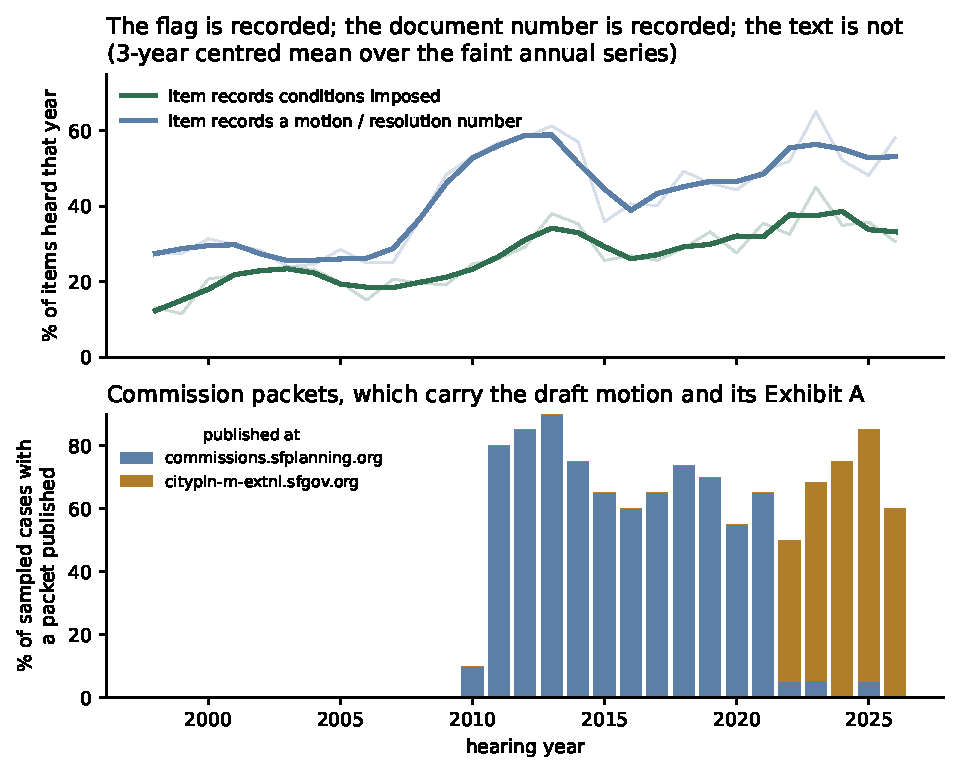
\includegraphics[width=\textwidth]{figures/fig_conditions_coverage.pdf}
\caption{Top: the share of items whose record carries the conditions flag and the share
carrying a motion, resolution or DRA number. Bottom: the share of a stratified random sample
of 20 cases per year for which a Commission packet is published, by host.}
\label{fig:coverage}
\end{figure}

\section{The minutes themselves: a negative result with evidence}

Before going outside the corpus it is worth testing whether the condition text is somewhere the
current schema is not looking. The item blocks are in \texttt{labels.db}
(\texttt{items.block\_text}) and are the same text the extraction read, so the sweep is free.

Table~\ref{tab:sweep} reports it over all 25{,}927 blocks. The minutes \emph{name} the
instrument often --- 23.1\% of blocks contain a motion, resolution or DRA number --- and
mention conditions of approval on 2.1\%. But blocks that both use condition language
\emph{and} carry an enumerated list number \textbf{15, or 0.06\%}. Reading all fifteen: they
are from 1998--2001, when the minutes were far more verbose, and every one is an
\emph{amendment} announced from the dais, of the form

\begin{quote}\small
\texttt{Conditions of Approval — ADD: 1) The proposed facility may include child-care services
for a maximum of 24 children. 3) The Project Sponsor shall provide at least one week's advance
notice of special events \dots}
\end{quote}

That is genuine condition text, and it is exactly what \texttt{modifications} captures. It is
not the conditions themselves. \textbf{The minutes are not a source for the standing
conditions of approval, and no better extraction of them would make it one.}

\section{DataSF: also not a source}

Two checks, both negative, both worth recording so they are not repeated.

\textbf{There is no commission-actions dataset.} Searching the DataSF catalogue returns 155
datasets matching ``planning''; none is a record of Commission decisions. The two Planning
Department Records tables in Table~\ref{tab:elsewhere} --- \texttt{y673-d69b} (Non-Projects)
and \texttt{qvu5-m3a2} (Projects) --- are \emph{application} records. They carry
record type, parcel, applicant, planner, open and close dates, a status, and for projects a
useful set of unit counts and an explicit \texttt{building\_permits} field. They do not carry
conditions, and they do not carry the Commission's action beyond a
\texttt{project\_decision} string. They are a good complement to the item table for other
purposes and no help at all for this one.

\textbf{DBI does not carry them either.} The last row of Table~\ref{tab:elsewhere} is the
test, computed by the same function the permit-linkage memo uses so the two cannot disagree:
DBI's \texttt{description} field is populated on 98.6\% of its 1{,}295{,}048 rows and
describes the \emph{work}; \textbf{87 rows --- 0.007\% ---} mention a condition of approval or
a Commission motion. A building department records the permit's scope and status, not the planning
conditions attached upstream of it.

\section{The Commission packet is the source, and it is addressable}

The document that carries the conditions is the \textbf{Commission packet}: the staff report
plus the \emph{draft motion}, whose \emph{Exhibit A --- Conditions of Approval, Compliance,
Monitoring, and Reporting} enumerates every condition and gives each a short name.

Two city hosts publish it, and neither covers the whole period:

\begin{itemize}
\item \texttt{commissions.sfplanning.org/cpcpackets/<case\_number>.pdf} --- keyed on the case
number alone. Covers roughly 2010--2021.
\item \texttt{citypln-m-extnl.sfgov.org/Commissions/CPC/<M>\_<D>\_<YYYY>/Commission\%20Packet/}
\texttt{<case\_number>.pdf} --- keyed on the case number \emph{under the hearing date}, which
the item table supplies. Covers 2022 onward.
\end{itemize}

Table~\ref{tab:packets} and the lower panel of Figure~\ref{fig:coverage} give availability on a
stratified random sample of 20 cases per hearing year, HEAD-probed against both. The result is
sharp:

\begin{itemize}
\item \textbf{1998--2009: 0 of 240 probed.} Nothing. The packet archive does not reach back that far,
and the pre-2010 half of the corpus is unreachable by this route.
\item \textbf{2011--2021: 55--90\% per year}, on the first host.
\item \textbf{2022--2026: 50--85\% per year}, on the second.
\end{itemize}

So the packet route covers \textbf{70.1\% of the 318 sampled cases heard from 2011 on, and
none of the 240 sampled before 2010} (Table~\ref{tab:packets}). That is a real constraint and it interacts badly with the corpus memo's central
pattern, which is a \emph{time series}: the conditioning share rose from 13.8\% in 1998 to
45.7\% in 2023, and the content of the conditions is observable only over the second half of
that span. Any claim about how the \emph{content} of conditions changed will be a claim about
2011 onwards.

\subsection{What the packet yields, by kind of case}
\label{sec:complement}

Table~\ref{tab:kinds} reports \textbf{every one of the 225 packets the probe found}, all of
them read; 106 carry a conditions section. The split by kind of case is sharp and it is not a
parser artefact:

\begin{itemize}
\item \textbf{Conditional use: 89 of 101 (88\%)}, with a median of \textbf{fifteen} numbered,
named conditions.
\item \textbf{Discretionary review: 1 of 41 (2\%).} Their packet is a ``Discretionary Review
Analysis'' --- a staff memo with no draft motion in it --- because a DR ends in a
Discretionary Review Action, not a conditioned authorisation. One was read end to end to
confirm: it contains no occurrence of ``conditions of approval'', ``Exhibit A'' or ``draft
motion''. The single exception, a mandatory DR of a cannabis dispensary, is instructive
rather than anomalous: staff recommended conditions on the \emph{use} there, so the packet
carries them.
\item \textbf{Environmental 0 of 7, legislative 1 of 25, variance 2 of 9.} None of these
families ends in a conditioned authorisation, and the three exceptions are prose about
conditions set by \emph{another} case's motion rather than a motion of their own --- which is
why Table~\ref{tab:kinds} reports the count of numbered conditions separately: all three
yield a heading and none yields a numbered list.
\item \textbf{`Other': 13 of 42.} A residual of downtown-project, office-allocation and
large-project authorisations, which \emph{are} conditioned authorisations. Their inclusion is
a reminder that the addressable set is not literally ``conditional use'' but ``any case that
ends in a motion''.
\end{itemize}

The pull is complete in the sense that matters: every packet the availability probe found has
been opened. Reaching the last of them needed two fixes worth recording, because both were
silently producing wrong answers rather than errors. \texttt{fetch} was deriving the hearing
date for the date-keyed URL differently from \texttt{probe} --- the earliest hearing of the
case rather than the earliest within the sampled year --- so for a case heard in two years it
built a URL that 404s; and a failed download was writing an empty file, which then read as
``this packet has no conditions''. Transport failures now leave no file, and ``read'' means
``a file exists'', so a packet that was never opened is excluded from the denominator instead
of counted as a negative.

This is the mirror image of the permit-linkage result, and the two memos should be read
together. \textbf{The permit route as the minutes print it reaches discretionary review
(83.8\% of DR items match a DBI permit) and essentially nothing else; the conditions route
reaches conditional use and essentially nothing else.}

\paragraph{Correction, 2026-09-08.} This paragraph originally continued: ``Between them they
cover most of the docket, but they never cover the same item, so an analysis that wants both
construction outcomes and condition content on one project cannot have them from these two
sources.'' \textbf{That is wrong, and the data-acquisition memo (\S3.3) shows why.} The claim
was about what the \emph{minutes} print, not about what is knowable. The Planning
Department's own records carry a \texttt{building\_permits} field, and following a conditional
use through it reaches a permit present in DBI on \textbf{46.0\% of the 5{,}074
conditional-use items} --- against the 0.3\% that print a permit number in the minutes. The
two routes do overlap, on nearly half of the conditional-use docket, and construction outcomes
and condition content \emph{can} be had on the same project.

A second constraint: the packet is published \emph{before} the hearing, so its motion is a
\textbf{draft} and its conditions are what staff proposed. What the Commission actually adopted
may differ, and the item table's \texttt{modifications} field is precisely the record of when
it did. The right reading is that the packet gives the proposed condition set and
\texttt{modifications} gives the Commission's amendments to it; neither alone is the adopted
motion.

\section{The conditions are templated}

Table~\ref{tab:titles} lists the most frequent condition headings across the packets read.
They yielded \textbf{216 distinct headings over 1{,}622 impositions} --- about 16 conditions
per motion, drawn from a vocabulary of a couple of hundred. The template is immediately
visible.
Conditions are numbered, named, and grouped under standing section headings --- Performance,
Design, Parking and Traffic, Provisions, Operation, Monitoring after Entitlement --- and the
names repeat across projects: \emph{Validity}, \emph{Expiration and Renewal}, \emph{Diligent
Pursuit}, \emph{Extension}, \emph{Conformity with Current Law}, \emph{Enforcement},
\emph{Revocation due to Violation of Conditions}, \emph{Transportation Sustainability Fee},
\emph{Bicycle Parking}, \emph{Sidewalk Maintenance}, \emph{Community Liaison}.

That is what makes a measure of burden feasible. If every motion wrote its conditions afresh,
converting them into indicators would be a document-understanding problem. Because they are
drawn from a standing template with a project-specific subset selected and project-specific
values filled in, the measurable object is \emph{which conditions were selected} --- a vector
of indicators --- with the free text reserved for the few that carry a number.

\section{A coding scheme, and how far it goes}
\label{sec:modifications}

\begin{figure}[htbp]\centering
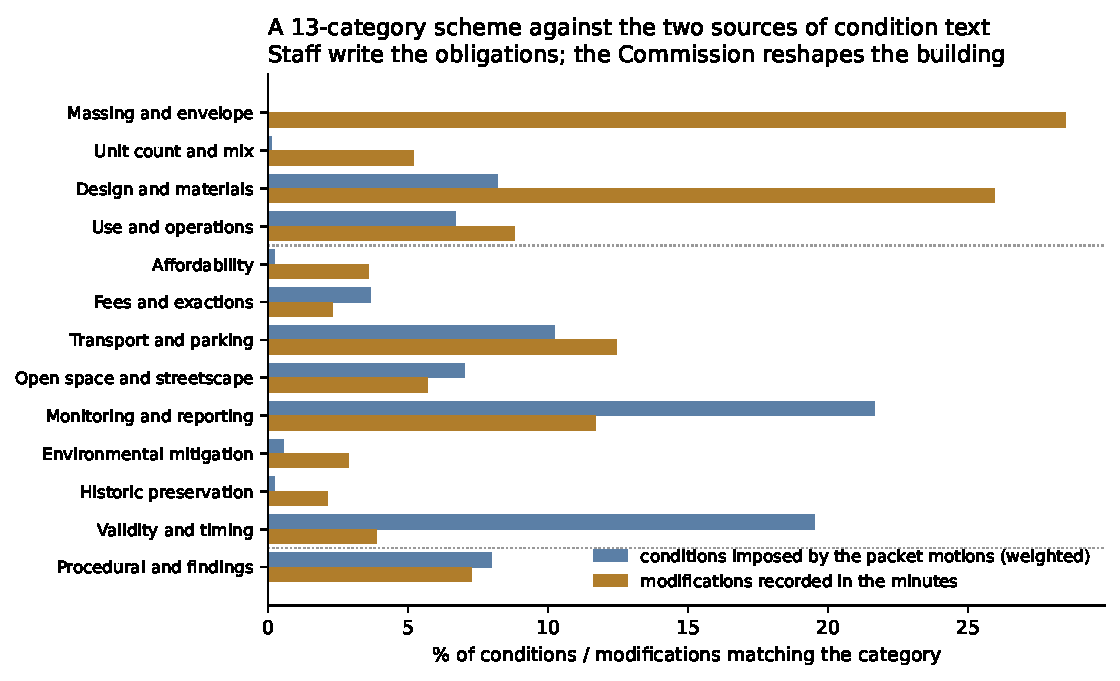
\includegraphics[width=\textwidth]{figures/fig_condition_taxonomy.pdf}
\caption{The thirteen categories against the two sources of condition text that exist: the
numbered condition headings of the packet motions, weighted by how often each heading is
imposed, and the \texttt{modifications} field of the item table. Dotted rules separate the
three families. The staff template is obligations; the Commission's amendments are the
building.}
\label{fig:taxonomy}
\end{figure}

Not every condition costs the same kind of money, and the distinction the paper needs is
between a condition that changes \emph{the project} and one that changes \emph{its
obligations}. The first shrinks or reshapes what gets built and shows up as forgone revenue;
the second leaves the building alone and attaches a payment, a duty or a monitoring regime, and
shows up as cost. \texttt{project\_modified} already flags the first family in principle, on
8.7\% of items.

Table~\ref{tab:taxonomy} sets out thirteen categories in three families:

\begin{description}
\item[Changes the project] massing and envelope; unit count and mix; design and materials; use
and operations.
\item[Changes its obligations] affordability; fees and exactions; transport and parking; open
space and streetscape; monitoring and reporting; environmental mitigation; historic
preservation; validity and timing.
\item[Neither] procedural findings --- the boilerplate a motion opens and closes with
(conformity with current law, General Plan consistency, severability, project description).
Kept separate so that ``covered by the scheme'' does not quietly take credit for procedural
furniture.
\end{description}

Applied to the two sources of text, the scheme reaches \textbf{85.6\% of the 1{,}622 condition
impositions} in the packets and \textbf{72.3\% of the 1{,}735 \texttt{modifications} texts}.
Coverage of \emph{distinct} headings is much lower, 58.8\%, and the gap is informative rather
than embarrassing: 58 of the 89 uncovered headings appear exactly once. The template is a small
recurring core plus a long tail of one-off, project-specific conditions, and no fixed scheme
will span the tail. Weighting by how often a condition is actually imposed is the right measure
of what a scheme reaches, and it is reported alongside the unweighted one in
Table~\ref{tab:taxonomy}. Both coverage figures moved by less than a point when the pull went
from 146 packets to all 225, which is the best evidence available that the vocabulary really
does saturate.

\textbf{The split between the two families is the substantive result.} Weighted by imposition,
\textbf{58.4\% of the packet conditions change the project's obligations and 12.8\% change the
project}; in the Commission's own \texttt{modifications} the proportions reverse, to 34.8\%
and 52.6\%. The detail is sharper still: \emph{massing and envelope} matches
\textbf{0.2\%} of packet conditions by imposition and 28.5\% of modifications. Staff's
conditions essentially never name heights and setbacks --- the building's shape is fixed by
the plans in Exhibit B, not by a named condition --- while more than a quarter of what the
Commission adds from the dais is exactly that. \textbf{Staff write the obligations; the
Commission reshapes the building.} That is a finding about who exercises which margin of
discretion, and it is invisible in a yes/no flag.

The two largest single categories in the staff template are \emph{monitoring and reporting}
(21.2\% of impositions) and \emph{validity and timing} (19.7\%) --- enforcement, revocation,
expiry, extension, diligent pursuit. \textbf{Two fifths of the conditions a project receives
are about the conditions themselves.} A further 14.9\% is procedural boilerplate, which is
why that family is scored apart: counting it as ``covered'' would flatter both the scheme and
the apparent burden.

\textbf{This coverage is in-sample and should be read as such.} The categories are hand-written
keyword patterns, drafted by reading the packet headings and a sample of the modifications
text, and then revised once against the headings the first draft missed. They were not revised
again, so the numbers above are one round of tuning away from naive, not zero --- but the claim
they support is the one the question asks, that a small scheme spans most of the vocabulary,
not that they constitute a validated classifier.

\section{What this establishes, and what is left}

\textbf{Established.}
\begin{enumerate}
\item The item table can say \emph{whether} but essentially never \emph{how}: the conditions
field is a three-character flag, and only \texttt{modifications} (10.7\% of items) holds
content.
\item The minutes are not a hidden source. 15 blocks in 25{,}927 enumerate a condition, all
from 1998--2001, all dais amendments.
\item Neither DataSF's planning records nor DBI's permit records carry conditions.
\item The Commission packet does, addressably, by case number on two hosts --- for 70.1\% of
sampled cases from 2011 on and none before 2010.
\item The packet route is a conditional-use instrument: 89 of 101 conditional-use packets carry
a conditions section against 1 of 41 discretionary reviews. This is the exact complement of the
permit route \emph{as the minutes print it} --- but not of the permit route as such: see the
correction in \S\ref{sec:complement}, which the data-acquisition memo forced.
\item The conditions are templated, named and enumerable, and a thirteen-category scheme spans
most of the observed vocabulary in both sources.
\end{enumerate}

\textbf{What is left.} Every packet the probe found has now been read, so the pull is
finished; what remains a sample is the \emph{probe}, which drew 20 cases per hearing year.
To go from here to an indicator matrix:

\begin{enumerate}
\item \textbf{Probe every case, not twenty a year.} 8{,}987 cases, of which the families that
end in a motion --- conditional use plus the downtown, office-allocation and large-project
authorisations that fall into `Other' in Table~\ref{tab:kinds} --- heard from 2011 on are the
addressable set. The probe is one or two HEAD requests per case and costs under an hour. The
pull is the expensive step and the cost is now measured rather than guessed: the 225 packets
here came to over 3\,GB, and the binding constraint is not bandwidth but
\texttt{pdfplumber}, which takes minutes per scanned plan set. Budget an overnight run,
resume it with \texttt{-{}-n}, and raise \texttt{-{}-max-mb} only for the tail.
\item \textbf{Extract to a condition list, not a blob.} The Exhibit A parser already recovers
numbered headings. The next step is one row per (case, condition number, heading, body), which
makes the count of conditions a variable in its own right --- the simplest measure of
stringency available, and one nothing in the current dataset can compute. The 225 packets read
here already carry \textbf{1{,}622 of them}.
\item \textbf{Validate against the minutes.} For items where the minutes record
\texttt{modifications}, the packet's proposed conditions and the Commission's amendments can be
compared directly. That is the only available check on whether the draft motion is a good proxy
for the adopted one, and it should be run before the draft is used as if it were.
\item \textbf{Hand-code a gold set.} The keyword scheme is a first pass. A few hundred
hand-coded conditions would let the categories be scored the way every other field in this
pipeline is scored, on a frozen split, with in-sample and out-of-sample reported separately.
\item \textbf{Accept the period.} No amount of work recovers condition content before 2010.
The measure will be a 2011--2026 measure, and the pre-2010 half of the corpus will have to be
carried on the flag alone. Saying so now is cheaper than discovering it in a regression.
\end{enumerate}

\section{Reproducing this}

\texttt{code/commission\_minutes\_processing/analyze\_conditions.py} runs in three stages, each
cached so neither network stage repeats by accident:

\begin{verbatim}
python analyze_conditions.py probe --per-year 20  # is a packet published?
python analyze_conditions.py fetch --n 225        # pull it, keep Exhibit A
python analyze_conditions.py fetch --max-mb 250   # ...the scanned ones too
python analyze_conditions.py report               # figures + tables
\end{verbatim}

\texttt{probe} writes \texttt{availability.csv} and \texttt{fetch} writes one text file per
case under \texttt{conditions/}, both in
\texttt{\$MFHR\_DATA\_ROOT/external/cpc\_packets/}; only the extracted conditions text is
kept, not the packets. \texttt{report} regenerates both figures and
\texttt{tables/condition\_tables.tex}. No number in this memo is hand-placed.

\end{document}
